\documentclass[11pt,a4paper]{article}

% --- Packages ---
\usepackage[utf8]{inputenc}
\usepackage[margin=0.8in,headheight=14.5pt]{geometry}
\usepackage{fancyhdr}
\usepackage{amsmath,amssymb}
\usepackage{booktabs}
\usepackage{tabularx}
\usepackage{ragged2e}
\usepackage{listings}
\usepackage{xcolor}
\usepackage{tikz}
\usepackage{pgfplots}
\usepackage{hyperref}
\usepackage{caption}
\usepackage{subcaption}
\usepackage{float}
\usepackage{microtype}
\usepackage{enumitem}
\usetikzlibrary{calc,shapes,arrows.meta,positioning,backgrounds,decorations.pathreplacing}
\pgfplotsset{compat=1.18}

% Prevent vertical stretching and minimize gaps around floats/lists
\raggedbottom
\setlist{itemsep=1.5pt, topsep=2.5pt, parsep=1pt, partopsep=0pt}
\setlength{\intextsep}{5pt plus 1pt minus 1pt}
\setlength{\textfloatsep}{5pt plus 1pt minus 1pt}
\setlength{\abovecaptionskip}{3pt}
\setlength{\belowcaptionskip}{2pt}
\setlength{\abovedisplayskip}{4pt plus 1pt minus 1pt}
\setlength{\belowdisplayskip}{4pt plus 1pt minus 1pt}

% Compact section spacing to prevent orphan breaks
\makeatletter
\renewcommand\section{\@startsection {section}{1}{\z@}%
                                   {-2.2ex \@plus -0.5ex \@minus -.2ex}%
                                   {1.2ex \@plus.2ex}%
                                   {\normalfont\Large\bfseries}}
\renewcommand\subsection{\@startsection{subsection}{2}{\z@}%
                                     {-1.8ex\@plus -0.4ex \@minus -.2ex}%
                                     {0.8ex \@plus .2ex}%
                                     {\normalfont\large\bfseries}}
\makeatother

% --- Hyperref Setup ---
\hypersetup{
    colorlinks=true,
    linkcolor=blue!70!black,
    citecolor=blue!70!black,
    urlcolor=blue!70!black
}

% --- Header and Footer ---
\pagestyle{fancy}
\fancyhf{}
\lhead{Medium Access Control: Code Division Multiple Access}
\rhead{Computer Networks Lab: Assignment 4}
\cfoot{Page \thepage}
\renewcommand{\headrulewidth}{0.4pt}
\renewcommand{\footrulewidth}{0.0pt}

% --- Code Listing Styling ---
\definecolor{codegreen}{rgb}{0,0.6,0}
\definecolor{codegray}{rgb}{0.45,0.45,0.45}
\definecolor{codepurple}{rgb}{0.58,0,0.82}
\definecolor{backcolour}{rgb}{0.96,0.97,0.98}
\definecolor{keycolor}{rgb}{0.0,0.2,0.6}

\lstdefinestyle{cstyle}{
    language=C,
    morekeywords={uint8_t,uint16_t,uint32_t,int16_t,size_t,EthernetFrame,sock_t,ClientSlot,MsgType},
    backgroundcolor=\color{backcolour},   
    commentstyle=\color{codegreen}\itshape,
    keywordstyle=\color{keycolor}\bfseries,
    numberstyle=\tiny\color{codegray},
    stringstyle=\color{codepurple},
    basicstyle=\ttfamily\scriptsize,
    breakatwhitespace=false,         
    breaklines=true,                 
    captionpos=b,                    
    keepspaces=true,                 
    numbers=left,                    
    numbersep=6pt,                  
    showspaces=false,                
    showstringspaces=false,
    showtabs=false,                  
    tabsize=4,
    frame=single,
    rulecolor=\color{black!20},
    columns=flexible,
    aboveskip=4pt,
    belowskip=4pt
}

\lstdefinestyle{tracestyle}{
    backgroundcolor=\color{backcolour},
    basicstyle=\ttfamily\scriptsize,
    columns=flexible,
    numbers=none,
    frame=single,
    rulecolor=\color{black!20},
    breaklines=true,
    keepspaces=true,
    aboveskip=4pt,
    belowskip=4pt
}

\lstset{style=cstyle}

\begin{document}

% =========================================================================
% COVER PAGE
% =========================================================================
\hypersetup{pageanchor=false}
\begin{titlepage}
    \centering
    \vspace*{1.2cm}
    
    {\Large \textbf{JADAVPUR UNIVERSITY}}\\[0.3cm]
    {\large DEPARTMENT OF COMPUTER SCIENCE AND ENGINEERING}\\[1.8cm]
    
    \rule{\linewidth}{1.2pt}\\[0.4cm]
    {\huge \textbf{Assignment 4 Report}}\\[0.3cm]
    {\LARGE \textbf{Design and Implementation of Code Division Multiple Access (CDMA) with Orthogonal Walsh-Hadamard Spreading Codes}}\\[0.3cm]
    {\large \textit{Mathematical Formulation, Linear Superposition Multiplexing, and End-to-End File Integrity Verification over a Simulated Socket Shared Channel}}\\[0.3cm]
    \rule{\linewidth}{1.2pt}\\[1.8cm]
    
    \begin{minipage}[t]{0.88\textwidth}
        \large
        \textbf{Course:} Computer Networks Laboratory (BCSE-III)\\[0.25cm]
        \textbf{Student Name:} Mandeep Shaw\\[0.25cm]
        \textbf{Section:} A1\\[0.25cm]
        \textbf{Roll Number:} 302510501002\\[0.25cm]
        \textbf{Assignment:} Assignment 4 (Medium Access Control: Code Division Multiple Access with Walsh Spreading Codes)\\[0.25cm]
        \textbf{Date of Submission:} November 2026
    \end{minipage}
    
    \vfill
    {\small Faculty of Engineering and Technology $\bullet$ Jadavpur University, Kolkata, India}
    \vspace*{0.8cm}
\end{titlepage}

% =========================================================================
% TABLE OF CONTENTS
% =========================================================================
\hypersetup{pageanchor=true}
\pagenumbering{roman}
\tableofcontents
\newpage
\pagenumbering{arabic}
\setcounter{page}{1}

% =========================================================================
% SECTION 1: INTRODUCTION AND OBJECTIVES
% =========================================================================
\section{Introduction and Objectives}
In shared physical communication channels, multiple independent network nodes must simultaneously communicate without destructive mutual interference. Medium Access Control (MAC) protocols fall into two broad taxonomies: \textbf{contention-based random access} (such as Pure ALOHA, Slotted ALOHA, CSMA, and CSMA/CD studied in Assignment 3) and \textbf{channel partitioning / channelization} techniques (such as Frequency Division Multiple Access (FDMA), Time Division Multiple Access (TDMA), and Code Division Multiple Access (CDMA)).

While contention-based schemes rely on probabilistic deferrals, carrier sensing, and collision resolution (which inherently degrade under heavy traffic due to collision cascades), \textbf{Code Division Multiple Access (CDMA)} multiplexes multiple concurrent transmissions onto the exact same frequency band at the exact same physical time instant without collision. CDMA achieves this by assigning each station a mutually orthogonal spreading sequence known as a \textbf{Walsh-Hadamard codeword}. Concurrent transmissions linearly superpose on the shared channel; at the receiving end, inner-product correlation with the target station's unique code filters out all other concurrent transmissions as complete mathematical zeros.

The primary objectives of this laboratory assignment are:
\begin{enumerate}
    \item \textbf{Emulation of a Shared CDMA Channel Server:} Design and construct a multi-client socket-based shared channel multiplexer in C running over TCP/IP loopback (\texttt{127.0.0.1:5000}) that coordinates synchronous time-slotted transmissions, aggregates incoming chip vectors, computes linear superposition, and broadcasts composite signals to the receiver.
    \item \textbf{Implementation of Walsh-Hadamard Code Generator:} Implement Sylvester's recursive construction algorithm to dynamically generate orthogonal Hadamard matrices of order $N = 2^{\lceil \log_2 n \rceil}$ for arbitrary station counts $n$.
    \item \textbf{Direct Sequence Spread Spectrum (DSSS) Station Transmitters:} Construct independent client processes emulating network interface cards (NICs). Stations segment arbitrary files into standard 46-byte payloads, encapsulate them into 65-byte Ethernet-style frames (520 bits), modulate data bits into bipolar chips ($\pm 1$), and spread each frame into $520 \times N$ chips.
    \item \textbf{Orthogonal Correlator Bank Receiver:} Construct a multi-channel receiver node that ingests composite chip streams, executes parallel inner-product correlation against all assigned Walsh codewords, demodulates bipolar values into clean bitstreams, reassembles 65-byte frames, and logs station idle states.
    \item \textbf{Empirical Evaluation across Mandatory Test Cases:} Rigorously benchmark and verify system behavior under five structured scenarios:
    \begin{itemize}
        \item \textbf{Test Case 1:} Non-Power-of-2 Stations (Matrix Expansion \& Zero-Padding, $n = 3 \implies N = 4$).
        \item \textbf{Test Case 2:} Unbalanced Payload Lengths (Dynamic Silence / Partial Transmissions, 10 KB vs. 1 KB).
        \item \textbf{Test Case 3:} Complementary Bit Pattern Stress (Extreme Channel Amplitude bounds of $\pm 4$ and $0$).
        \item \textbf{Test Case 4:} Complete File Integrity Verification (Bit-for-bit diff and cryptographic MD5/SHA-256 checks).
        \item \textbf{Test Case 5:} Higher Spreading Factor Scaling ($N = 8$, 4160 chips/frame, 5 parallel streams).
    \end{itemize}
\end{enumerate}

% =========================================================================
% SECTION 2: THEORETICAL PRINCIPLES OF CDMA
% =========================================================================
\section{Theoretical Principles of Code Division Multiple Access}

\subsection{Direct Sequence Spread Spectrum (DSSS) and Spreading Factor}
In Direct Sequence Spread Spectrum (DSSS), the baseband transmission bandwidth is deliberately spread over a significantly wider spectral frequency band by multiplying each information bit by a high-rate pseudorandom or orthogonal sequence of $N$ binary pulses called \textbf{chips}. 

Let $T_b$ denote the bit duration and $T_c$ denote the chip duration. The ratio defines the \textbf{Spreading Factor} (also referred to as Processing Gain $G_p$):
\begin{equation}
    N = \frac{T_b}{T_c}
\end{equation}
For a baseband frame containing $L_{\text{frame}} = 65\text{ bytes} = 520\text{ bits}$, the total number of serialized chips emitted onto the physical medium per frame is:
\begin{equation}
    C_{\text{frame}} = L_{\text{frame}} \times 8 \times N = 520 \times N \text{ chips}
\end{equation}
When $N = 2$, each frame spans 1,040 chips; for $N = 4$, 2,080 chips; and for $N = 8$, 4,160 chips.

\subsection{Walsh-Hadamard Codes and Sylvester's Construction}
Walsh codes are mutually orthogonal binary sequences whose values are drawn from $\{-1, +1\}$. A Walsh-Hadamard matrix $\mathbf{H}_N$ of dimension $N \times N$ (where $N = 2^k, k \in \mathbb{N}$) is generated recursively via \textbf{Sylvester's construction}:
\begin{equation}
    \mathbf{H}_1 = [1], \qquad \mathbf{H}_{2k} = \begin{bmatrix} \mathbf{H}_k & \mathbf{H}_k \\ \mathbf{H}_k & -\mathbf{H}_k \end{bmatrix}
\end{equation}
For $N = 2$:
\begin{equation}
    \mathbf{H}_2 = \begin{bmatrix} +1 & +1 \\ +1 & -1 \end{bmatrix} \implies \begin{cases} \mathbf{W}_0 = [+1, +1] \\ \mathbf{W}_1 = [+1, -1] \end{cases}
\end{equation}
For $N = 4$:
\begin{equation}
    \mathbf{H}_4 = \begin{bmatrix} 
        +1 & +1 & +1 & +1 \\ 
        +1 & -1 & +1 & -1 \\ 
        +1 & +1 & -1 & -1 \\ 
        +1 & -1 & -1 & +1 
    \end{bmatrix} \implies \begin{cases} 
        \mathbf{W}_0 = [+1, +1, +1, +1] \\ 
        \mathbf{W}_1 = [+1, -1, +1, -1] \\ 
        \mathbf{W}_2 = [+1, +1, -1, -1] \\ 
        \mathbf{W}_3 = [+1, -1, -1, +1] 
    \end{cases}
\end{equation}
For $N = 8$, the recursive construction yields an $8 \times 8$ matrix where each of the 8 row vectors $\mathbf{W}_0 \dots \mathbf{W}_7$ contains 8 chips.

\subsection{Orthogonality and Normalized Cross-Correlation}
The fundamental mathematical property enabling collision-free multi-user separation is the \textbf{zero cross-correlation} between distinct rows of $\mathbf{H}_N$. The discrete inner product between any two Walsh sequence vectors $\mathbf{W}_i$ and $\mathbf{W}_j$ satisfies:
\begin{equation}
    \frac{1}{N} (\mathbf{W}_i \cdot \mathbf{W}_j) = \frac{1}{N} \sum_{c=0}^{N-1} w_{i,c} w_{j,c} = \delta_{ij} = \begin{cases} 1, & \text{if } i = j \quad \text{(Normalized Autocorrelation)} \\ 0, & \text{if } i \ne j \quad \text{(Zero Cross-Correlation)} \end{cases}
\end{equation}
where $\delta_{ij}$ represents the Kronecker delta.

\subsection{Channel Superposition and Correlator Demodulation}
To transmit binary data over the physical medium, each raw data bit $b_i \in \{0, 1\}$ of station $i$ is first mapped to a bipolar symbol $d_i \in \{-1, +1\}$:
\begin{equation}
    d_i = \begin{cases} +1, & \text{if } b_i = 1 \\ -1, & \text{if } b_i = 0 \end{cases}
\end{equation}
The station modulates its assigned Walsh codeword $\mathbf{W}_i$ by $d_i$, producing chip sequence $\mathbf{C}_i = d_i \mathbf{W}_i$.

When $n$ stations transmit simultaneously on the shared medium during the same synchronous slot, the physical channel acts as a linear adder. The composite channel chip signal $\mathbf{S}$ is the algebraic sum of all active transmitted waveforms:
\begin{equation}
    \mathbf{S} = \sum_{i=0}^{n-1} d_i \mathbf{W}_i = d_0 \mathbf{W}_0 + d_1 \mathbf{W}_1 + \dots + d_{n-1} \mathbf{W}_{n-1}
\end{equation}
At the destination receiver node, extracting the specific bit transmitted by target station $k$ requires computing the normalized inner product between the composite signal $\mathbf{S}$ and the target station's unique Walsh vector $\mathbf{W}_k$:
\begin{align}
    \frac{1}{N} (\mathbf{S} \cdot \mathbf{W}_k) &= \frac{1}{N} \left( \sum_{i=0}^{n-1} d_i \mathbf{W}_i \right) \cdot \mathbf{W}_k \nonumber \\
    &= \sum_{i=0}^{n-1} d_i \left( \frac{1}{N} \mathbf{W}_i \cdot \mathbf{W}_k \right) \nonumber \\
    &= \sum_{i=0}^{n-1} d_i \delta_{ik} = d_k
\end{align}
Because all interfering cross-terms identically vanish ($\frac{1}{N} \mathbf{W}_i \cdot \mathbf{W}_k = 0$ for all $i \ne k$), the inner product yields $d_k$ with zero multi-user interference (MUI). The decision rule recovers the original data bit:
\begin{equation}
    \hat{b}_k = \begin{cases} 1, & \text{if } d_k = +1 \\ 0, & \text{if } d_k = -1 \\ \text{Idle / Silent}, & \text{if } d_k = 0 \end{cases}
\end{equation}

\subsection{Matrix Expansion, Zero-Padding, and Dynamic Silence}
When the number of contending stations $n$ is not an exact power of 2, the system rounds up to the next power of 2:
\begin{equation}
    N = 2^{\lceil \log_2 n \rceil}
\end{equation}
For example, with $n = 3$ stations, the server instantiates an $N = 4$ Hadamard matrix. Stations 0, 1, and 2 are assigned codes $\mathbf{W}_0, \mathbf{W}_1, \mathbf{W}_2$. Code $\mathbf{W}_3$ remains unused ($d_3 = 0$). 
Because $\mathbf{W}_3$ is strictly orthogonal to $\mathbf{W}_0, \mathbf{W}_1, \mathbf{W}_2$, correlating against $\mathbf{W}_3$ produces:
\begin{equation}
    \frac{1}{4} (\mathbf{S} \cdot \mathbf{W}_3) = \frac{1}{4} (d_0 \mathbf{W}_0 + d_1 \mathbf{W}_1 + d_2 \mathbf{W}_2) \cdot \mathbf{W}_3 = 0 \implies \text{Silent Channel}
\end{equation}
Similarly, when a station finishes transmitting early (e.g., Station 2 finishing after 22 frames while Station 1 continues for 220 frames), the server treats the finished station as silent ($d_2 = 0$). In subsequent slots:
\begin{equation}
    \mathbf{S} = d_1 \mathbf{W}_1 + 0 \cdot \mathbf{W}_2 = d_1 \mathbf{W}_1
\end{equation}
The receiver computes $\frac{1}{2}(\mathbf{S} \cdot \mathbf{W}_1) = d_1$ and $\frac{1}{2}(\mathbf{S} \cdot \mathbf{W}_2) = 0$, guaranteeing uninterrupted lossless communication.

% =========================================================================
% SECTION 3: SYSTEM ARCHITECTURE AND PROCEDURAL DESIGN
% =========================================================================
\section{System Architecture and Procedural Design}

\subsection{3-Tier Client-Server Architecture Overview}
The CDMA emulation environment is organized as a modular 3-tier client-server pipeline operating over TCP/IP loopback (\texttt{127.0.0.1:5000}):
\begin{itemize}
    \item \textbf{Contending Network Stations (\texttt{sender.c}):} Independent processes representing network nodes. Each station connects to the channel server, registers its unique name, receives its assigned Walsh codeword $\mathbf{W}_i$, segments arbitrary input files into 46-byte payloads, constructs 65-byte Ethernet frames, encodes frame bits into bipolar chips, dispatches chip packets, and awaits slot acknowledgments.
    \item \textbf{Shared Channel Server (\texttt{server.c}):} Acts as the physical medium and linear superposition arbiter. It accepts registrations from $n$ stations and the receiver, generates the $N \times N$ Walsh matrix, assigns orthogonal codes, synchronizes time slots, superposes incoming chip streams element-wise into a single composite vector $\mathbf{S}$, dispatches $\mathbf{S}$ to the receiver, and relays slot ACKs back to active stations.
    \item \textbf{Destination Receiver Node (\texttt{receiver.c}):} Connects to the server, ingests composite chip streams, maintains a parallel correlator bank for all $N$ Walsh codes, extracts clean frames, verifies checksums, writes station-specific reconstructed payload files (\texttt{output\_station\_X.txt}), and returns slot acknowledgments.
\end{itemize}

\begin{figure}[H]
    \centering
    \resizebox{0.88\textwidth}{!}{%
    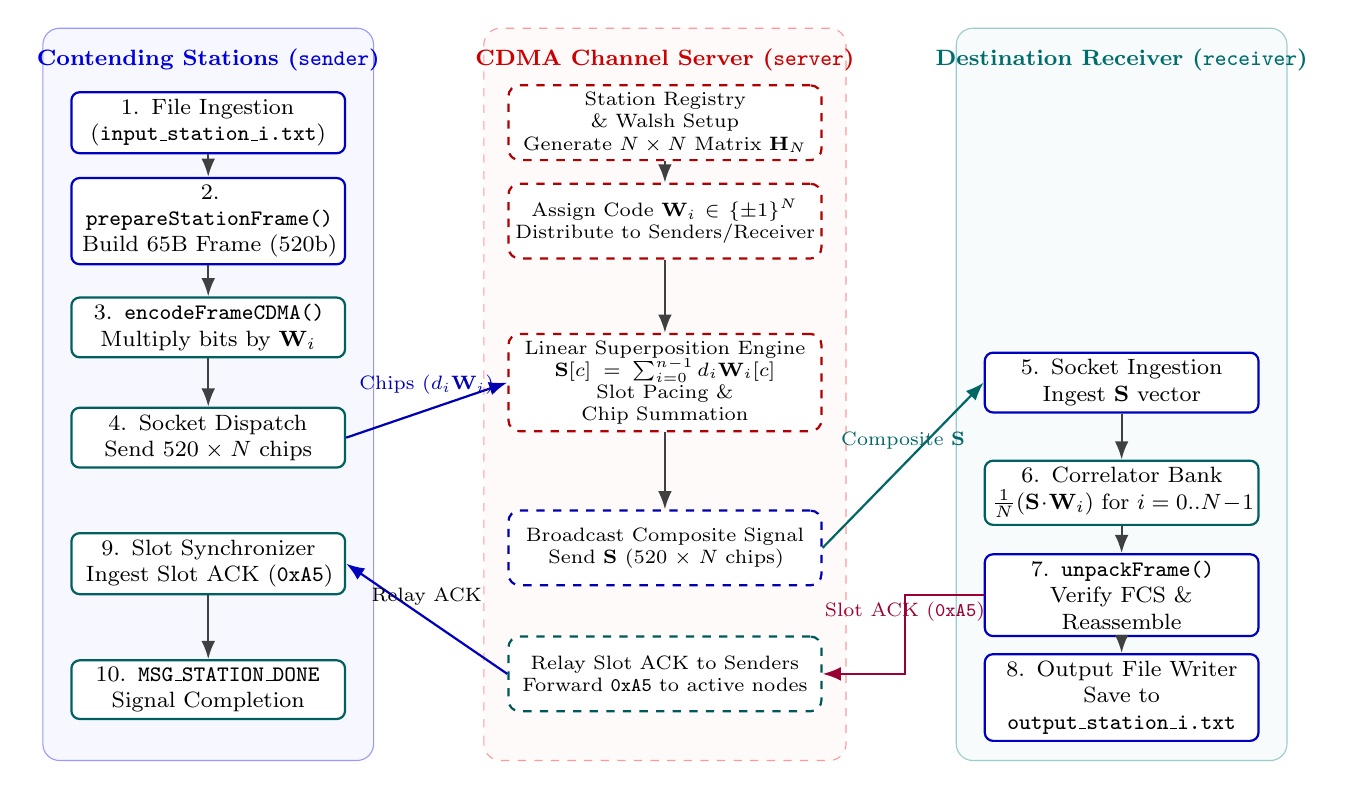
\begin{tikzpicture}[
        font=\footnotesize,
        >=Latex,
        block/.style={rectangle, draw=blue!75!black, fill=white, thick, rounded corners=3pt, minimum height=0.72cm, text width=3.3cm, align=center, inner sep=2.5pt},
        proc/.style={rectangle, draw=teal!75!black, fill=white, thick, rounded corners=3pt, minimum height=0.72cm, text width=3.3cm, align=center, inner sep=2.5pt},
        chan/.style={rectangle, draw=red!70!black, fill=white, thick, dashed, rounded corners=4pt, minimum height=0.95cm, text width=3.8cm, align=center, font=\scriptsize, inner sep=2.5pt},
        arrow/.style={->, thick, draw=black!75},
        retarrow/.style={->, thick, draw=blue!75!black}
    ]
        % Background Containers
        \begin{scope}[on background layer]
            \draw[draw=blue!40, fill=blue!3, rounded corners=6pt] (-0.4, -4.5) rectangle (3.8, 4.8);
            \draw[draw=red!40, fill=red!2, dashed, rounded corners=6pt] (5.2, -4.5) rectangle (9.8, 4.8);
            \draw[draw=teal!40, fill=teal!3, rounded corners=6pt] (11.2, -4.5) rectangle (15.4, 4.8);
        \end{scope}

        % Header Labels
        \node[font=\bfseries\footnotesize, text=blue!85!black] at (1.7, 4.4) {Contending Stations (\texttt{sender})};
        \node[font=\bfseries\footnotesize, text=red!80!black]  at (7.5, 4.4) {CDMA Channel Server (\texttt{server})};
        \node[font=\bfseries\footnotesize, text=teal!85!black] at (13.3, 4.4) {Destination Receiver (\texttt{receiver})};

        % Senders
        \node[block] (s_read)  at (1.7, 3.6)  {1. File Ingestion\\(\texttt{input\_station\_i.txt})};
        \node[block] (s_frame) at (1.7, 2.35) {2. \texttt{prepareStationFrame()}\\Build 65B Frame (520b)};
        \node[proc]  (s_cdma)  at (1.7, 1.0)  {3. \texttt{encodeFrameCDMA()}\\Multiply bits by $\mathbf{W}_i$};
        \node[proc]  (s_send)  at (1.7, -0.4) {4. Socket Dispatch\\Send $520 \times N$ chips};
        \node[proc]  (s_ack)   at (1.7, -2.0) {9. Slot Synchronizer\\Ingest Slot ACK (\texttt{0xA5})};
        \node[proc]  (s_done)  at (1.7, -3.6) {10. \texttt{MSG\_STATION\_DONE}\\Signal Completion};

        % Server
        \node[chan] (c_reg)   at (7.5, 3.6)  {Station Registry \& Walsh Setup\\Generate $N \times N$ Matrix $\mathbf{H}_N$};
        \node[chan] (c_assign)at (7.5, 2.35) {Assign Code $\mathbf{W}_i \in \{\pm 1\}^N$\\Distribute to Senders/Receiver};
        \node[chan] (c_super) at (7.5, 0.3)  {Linear Superposition Engine\\$\mathbf{S}[c] = \sum_{i=0}^{n-1} d_i \mathbf{W}_i[c]$\\Slot Pacing \& Chip Summation};
        \node[chan, draw=blue!70!black] (c_fwd) at (7.5, -1.8) {Broadcast Composite Signal\\Send $\mathbf{S}$ ($520 \times N$ chips)};
        \node[chan, draw=teal!70!black] (c_ack) at (7.5, -3.4) {Relay Slot ACK to Senders\\Forward \texttt{0xA5} to active nodes};

        % Receiver
        \node[block] (r_recv)   at (13.3, 0.3)  {5. Socket Ingestion\\Ingest $\mathbf{S}$ vector};
        \node[proc]  (r_corr)   at (13.3, -1.1) {6. Correlator Bank\\$\frac{1}{N}(\mathbf{S} \cdot \mathbf{W}_i)$ for $i=0..N-1$};
        \node[block] (r_unpack) at (13.3, -2.4) {7. \texttt{unpackFrame()}\\Verify FCS \& Reassemble};
        \node[block] (r_out)    at (13.3, -3.7) {8. Output File Writer\\Save to \texttt{output\_station\_i.txt}};

        % Arrows
        \draw[arrow] (s_read) -- (s_frame);
        \draw[arrow] (s_frame) -- (s_cdma);
        \draw[arrow] (s_cdma) -- (s_send);

        \draw[arrow, blue!70!black] (s_send.east) -- node[above=2pt, font=\scriptsize] {Chips ($d_i \mathbf{W}_i$)} (c_super.west);
        \draw[arrow] (c_reg) -- (c_assign);
        \draw[arrow] (c_assign) -- (c_super);
        \draw[arrow] (c_super) -- (c_fwd);

        \draw[arrow, teal!80!black] (c_fwd.east) -- node[above=2pt, font=\scriptsize] {Composite $\mathbf{S}$} (r_recv.west);
        \draw[arrow] (r_recv) -- (r_corr);
        \draw[arrow] (r_corr) -- (r_unpack);
        \draw[arrow] (r_unpack) -- (r_out);

        \draw[arrow, purple!80!black] (r_unpack.west) -- ++(-1.0, 0) |- node[pos=0.25, above=1pt, font=\scriptsize] {Slot ACK (\texttt{0xA5})} (c_ack.east);
        \draw[retarrow] (c_ack.west) -- node[above=1pt, font=\scriptsize] {Relay ACK} (s_ack.east);
        \draw[arrow] (s_ack) -- (s_done);
    \end{tikzpicture}}
    \caption{Three-tier procedural organization of the synchronous multi-station CDMA shared channel system.}
    \label{fig:arch_overview}
\end{figure}

\subsection{Frame Structure and Chip Spreading Serialization}
Conforming strictly to preceding lab assignments, every transmission uses a fixed 65-byte Ethernet-style frame consisting of a 15-byte header, a 46-byte payload, and a 4-byte Frame Check Sequence (FCS) trailer, totaling $65 \times 8 = 520\text{ bits}$.

\begin{figure}[H]
    \centering
    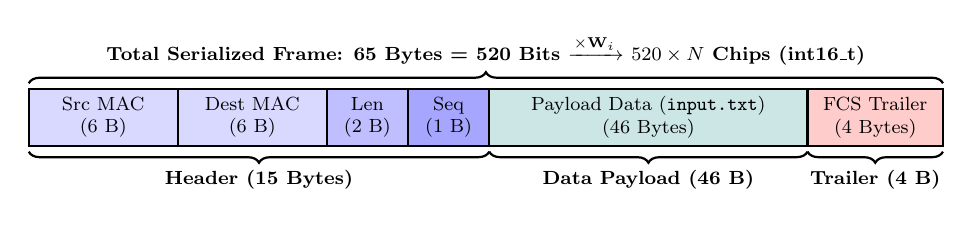
\begin{tikzpicture}[font=\footnotesize, scale=0.86, every node/.style={transform shape}]
        % Header blocks
        \draw[fill=blue!15, thick] (0,0) rectangle (2.2, 0.85) node[pos=0.5, align=center] {Src MAC\\(6 B)};
        \draw[fill=blue!15, thick] (2.2,0) rectangle (4.4, 0.85) node[pos=0.5, align=center] {Dest MAC\\(6 B)};
        \draw[fill=blue!25, thick] (4.4,0) rectangle (5.6, 0.85) node[pos=0.5, align=center] {Len\\(2 B)};
        \draw[fill=blue!35, thick] (5.6,0) rectangle (6.8, 0.85) node[pos=0.5, align=center] {Seq\\(1 B)};

        % Payload block
        \draw[fill=teal!20, thick] (6.8,0) rectangle (11.5, 0.85) node[pos=0.5, align=center] {Payload Data (\texttt{input.txt})\\(46 Bytes)};

        % Trailer block
        \draw[fill=red!20, thick] (11.5,0) rectangle (13.5, 0.85) node[pos=0.5, align=center] {FCS Trailer\\(4 Bytes)};

        % Braces and labels
        \draw[decorate, decoration={brace, mirror, amplitude=4pt}, thick] (0,-0.08) -- (6.8,-0.08)
            node[pos=0.5, below=4pt] {\textbf{Header (15 Bytes)}};
        \draw[decorate, decoration={brace, mirror, amplitude=4pt}, thick] (6.8,-0.08) -- (11.5,-0.08)
            node[pos=0.5, below=4pt] {\textbf{Data Payload (46 B)}};
        \draw[decorate, decoration={brace, mirror, amplitude=4pt}, thick] (11.5,-0.08) -- (13.5,-0.08)
            node[pos=0.5, below=4pt] {\textbf{Trailer (4 B)}};
        \draw[decorate, decoration={brace, amplitude=4pt}, thick] (0,0.93) -- (13.5,0.93)
            node[pos=0.5, above=4pt] {\textbf{Total Serialized Frame: 65 Bytes = 520 Bits $\xrightarrow{\times \mathbf{W}_i}$ $520 \times N$ Chips (int16\_t)}};
    \end{tikzpicture}
    \caption{In-memory layout and bit-to-chip expansion of the 65-byte Data Link Frame.}
    \label{fig:frame_layout}
\end{figure}

The acknowledgment frame is compact (2 bytes):
\begin{equation}
    \text{Slot ACK Frame} = [\text{Marker (\texttt{0xA5})} \ (1\text{ Byte}) \mid \text{Slot Sequence Number} \ (1\text{ Byte})]
\end{equation}

\subsection{Protocol Opcodes and Channel Handshake}
The entities coordinate through standardized control opcodes defined in \texttt{csma\_common.h}:
\begin{itemize}
    \item \texttt{MSG\_REGISTER\_RX} (\texttt{0x01}): Destination receiver registers with the channel server.
    \item \texttt{MSG\_RX\_INIT} (\texttt{0x02}): Server sends configuration header to receiver: $[n, N, \text{stationNames}\dots]$.
    \item \texttt{MSG\_REGISTER} (\texttt{0x05}): Sender station registers its 32-byte name string.
    \item \texttt{MSG\_ASSIGN\_WALSH} (\texttt{0x06}): Server transmits station ID, station count $n$, and Walsh dimension $N$.
    \item \texttt{MSG\_CDMA\_FRAME} (\texttt{0x20}): Sender dispatches sequence number and $520 \times N$ encoded chips.
    \item \texttt{MSG\_COMPOSITE\_SIG} (\texttt{0x30}): Server forwards composite summed chips to the receiver.
    \item \texttt{MSG\_TX\_ACK} (\texttt{0xA5}): Receiver returns slot ACK, which server relays to all active stations.
    \item \texttt{MSG\_STATION\_DONE} (\texttt{0xFF}): Station signals end of file; server marks station silent and shuts down gracefully.
\end{itemize}

% =========================================================================
% SECTION 4: IMPLEMENTATION DETAILS
% =========================================================================
\section{Implementation Details}

\subsection{Key Methods and Interfaces}
Table \ref{tab:methods} maps the programmatic methods implemented across the three software modules.

\begin{table}[H]
    \centering
    \small
    \begin{tabularx}{\textwidth}{llX}
        \toprule
        \textbf{Entity} & \textbf{Method Name} & \textbf{Functional Description} \\
        \midrule
        \texttt{sender.c} & \texttt{encodeFrameCDMA()} & Maps 520 frame bits to $\pm 1$ bipolar symbols and multiplies each bit by station's assigned $N$-chip Walsh vector $\mathbf{W}_i$. \\
        & \texttt{prepareStationFrame()} & Formats 65-byte Ethernet frame with MAC addressing, sequence number, and 46-byte payload. \\
        & \texttt{main()} & Connects to server, registers, receives $\mathbf{W}_i$, transmits chips per slot, awaits slot ACK, and sends \texttt{MSG\_STATION\_DONE}. \\
        \midrule
        \texttt{server.c} & \texttt{generateWalshTable()} & Implements Sylvester's recursive expansion to generate $N \times N$ Hadamard matrix. \\
        & \texttt{next\_power\_of\_2()} & Computes smallest power of 2 $N \ge n$ ($N = 2^{\lceil \log_2 n \rceil}$). \\
        & Synchronous Loop & Aggregates chip vectors from all non-finished stations, executes linear superposition $\mathbf{S}[c] = \sum d_i \mathbf{W}_i[c]$, broadcasts $\mathbf{S}$ to receiver, and relays ACKs. \\
        \midrule
        \texttt{receiver.c} & \texttt{decodeStationCDMA()} & Computes normalized inner product $\frac{1}{N}(\mathbf{S} \cdot \mathbf{W}_i)$ across all $N$ channels. Reconstructs frame if active, or flags channel idle if correlation is 0. \\
        & \texttt{unpackFrame()} & Deserializes 65-byte buffer, parses headers, and checks payload length. \\
        & File Output Writer & Appends reconstructed payload bytes to \texttt{output\_station\_X.txt} for end-to-end diff and hash verification. \\
        \bottomrule
    \end{tabularx}
    \caption{Functional mapping of sender, server, and receiver methods.}
    \label{tab:methods}
\end{table}

\subsection{Core Code Snippets}
Listing \ref{lst:walsh_encode} demonstrates Sylvester's recursive Hadamard construction and station frame chip encoding:

\begin{lstlisting}[style=cstyle, caption={Sylvester's recursive construction and DSSS chip spreading.}, label={lst:walsh_encode}]
/* csma_common.h: Sylvester's Recursive Hadamard Matrix Construction */
static inline void generateWalshTable(int N, int table[MAX_WALSH_SIZE][MAX_WALSH_SIZE]) {
    table[0][0] = 1;
    for (int len = 1; len < N; len <<= 1) {
        for (int i = 0; i < len; i++) {
            for (int j = 0; j < len; j++) {
                table[i][j + len]       =  table[i][j];
                table[i + len][j]       =  table[i][j];
                table[i + len][j + len] = -table[i][j];
            }
        }
    }
}

/* sender.c: Spread 65-byte Frame (520 bits) using Assigned Walsh Codeword */
static void encodeFrameCDMA(const unsigned char packedBuf[FRAME_SIZE],
                            const int walshCode[], int walshN, int16_t chipsOut[]) {
    int chipIdx = 0;
    for (int byteIdx = 0; byteIdx < FRAME_SIZE; byteIdx++) {
        unsigned char b = packedBuf[byteIdx];
        for (int bitIdx = 7; bitIdx >= 0; bitIdx--) {
            int bitVal = (b >> bitIdx) & 1;
            int bipolar = (bitVal == 1) ? 1 : -1;
            for (int c = 0; c < walshN; c++) {
                chipsOut[chipIdx++] = (int16_t)(bipolar * walshCode[c]);
            }
        }
    }
}
\end{lstlisting}

Listing \ref{lst:server_super_recv_decode} illustrates server superposition and receiver correlator decoding:

\begin{lstlisting}[style=cstyle, caption={Channel linear superposition and receiver inner-product correlation.}, label={lst:server_super_recv_decode}]
/* server.c: Linear Superposition of Chips across Simultaneously Transmitting Stations */
memset(compositeSignal, 0, chipBytes);
for (int i = 0; i < expected_stations; i++) {
    if (clients[i].has_slot_data) {
        for (int c = 0; c < totalChips; c++) {
            compositeSignal[c] += clients[i].chips[c];
        }
        total_frames_multiplexed++;
    }
}

/* receiver.c: Inner-Product Correlator Demodulator for Station Walsh Code W_i */
static int decodeStationCDMA(const int16_t compositeChips[], const int walshCode[],
                             int walshN, unsigned char packedBuf[FRAME_SIZE]) {
    memset(packedBuf, 0, FRAME_SIZE);
    int chipIdx = 0;
    for (int byteIdx = 0; byteIdx < FRAME_SIZE; byteIdx++) {
        unsigned char decodedByte = 0;
        for (int bitIdx = 7; bitIdx >= 0; bitIdx--) {
            int sum = 0;
            for (int c = 0; c < walshN; c++) {
                sum += (int)compositeChips[chipIdx++] * walshCode[c];
            }
            int bipolar = sum / walshN;
            /* If correlation is 0 on initial bit, station was silent/idle this slot */
            if (byteIdx == 0 && bitIdx == 7 && bipolar == 0) return 0;
            if (bipolar > 0) decodedByte |= (1 << bitIdx);
        }
        packedBuf[byteIdx] = decodedByte;
    }
    return 1;
}
\end{lstlisting}

% =========================================================================
% SECTION 5: TEST CASES AND EXPERIMENTAL METHODOLOGY
% =========================================================================
\section{Test Cases and Experimental Methodology}
To empirically validate the CDMA system against all laboratory specifications, five distinct test scenarios were executed:
\begin{enumerate}
    \item \textbf{Test Case 1: Non-Power-of-2 Stations (Matrix Expansion \& Zero-Padding):}
    \begin{itemize}
        \item \textit{Objective:} Verify that when $n = 3$, the system rounds up to $N = 4$ ($N = 2^{\lceil \log_2 3 \rceil}$), assigning $\mathbf{W}_0, \mathbf{W}_1, \mathbf{W}_2$ to active stations, while unused code $\mathbf{W}_3$ acts as a silent channel without affecting active stations.
        \item \textit{Setup:} Run \texttt{./server 3}, \texttt{./receiver 0}, and 3 senders (\texttt{Station\_1}, \texttt{Station\_2}, \texttt{Station\_3}).
        \item \textit{Expected Result:} $\mathbf{W}_3$ remains unused. Composite chips sum 3 stations (e.g., $[-3, -1, -1, +1]$). Correlating against $\mathbf{W}_3$ yields $\frac{1}{4}(\mathbf{S} \cdot \mathbf{W}_3) = 0 \implies \text{Silent/Idle}$. Stations 0, 1, 2 decode with 100\% accuracy.
    \end{itemize}

    \item \textbf{Test Case 2: Unbalanced Payload Lengths (Dynamic Silence / Partial Transmissions):}
    \begin{itemize}
        \item \textit{Objective:} Test channel behavior when contending stations finish at different times.
        \item \textit{Setup:} Station 1 transmits a 10 KB file (220 frames); Station 2 transmits a 1 KB file (22 frames).
        \item \textit{Expected Result:} Slots 1 to 22 superpose both stations ($\mathbf{S} = d_1 \mathbf{W}_1 + d_2 \mathbf{W}_2$). At slot 22, Station 2 sends \texttt{MSG\_STATION\_DONE} and disconnects. For slots 23 to 220, Station 2 is treated as silent ($0 \times \mathbf{W}_2$), and receiver logs \texttt{[Station \#1] Inner Product = 0 (Station Idle in Slot \#X)} while Station 1 continues receiving frames without corruption.
    \end{itemize}

    \item \textbf{Test Case 3: Complementary Bit Pattern Stress (Extreme Channel Amplitude):}
    \begin{itemize}
        \item \textit{Objective:} Verify dynamic range and arithmetic overflow in chip buffers when all stations transmit identical versus complementary bits.
        \item \textit{Setup:} 
        (a) All Ones Test: \texttt{0xFF} across 4 stations ($d_i = +1$).
        (b) All Zeros Test: \texttt{0x00} across 4 stations ($d_i = -1$).
        (c) Alternating Test: Station 1 sends \texttt{0xFF}, Station 2 sends \texttt{0x00}.
        \item \textit{Expected Result:} All Ones ($n = 4$) reaches peaks of $+4$ or $-4$ without 16-bit integer overflow. Alternating cancels signals along orthogonal chips producing frequent zeros. Receiver resolves all original bytes without corruption.
    \end{itemize}

    \item \textbf{Test Case 4: Complete File Integrity Verification (Hash / Diff Check):}
    \begin{itemize}
        \item \textit{Objective:} Prove end-to-end mathematical lossless reconstruction over the shared channel.
        \item \textit{Setup:} 4 stations transmit distinct, substantial payloads (35 frames each, 1,610 bytes each). Receiver writes decoded payloads to \texttt{output\_station\_X.txt}.
        \item \textit{Verification:} Execute \texttt{diff input\_station\_X.txt output\_station\_X.txt} and compare MD5 / SHA-256 cryptographic hashes.
        \item \textit{Expected Result:} \texttt{diff} produces exit code 0 (no differences). Hashes match 100\% bit-for-bit.
    \end{itemize}

    \item \textbf{Test Case 5: Higher Spreading Factor Scaling ($N = 8$):}
    \begin{itemize}
        \item \textit{Objective:} Validate Sylvester's expansion to larger matrices and higher chip counts ($520 \times 8 = 4,160\text{ chips/frame}$).
        \item \textit{Setup:} Run server with 5 stations: \texttt{./server 5} (expands to $N = 8$). Launch 5 senders.
        \item \textit{Expected Result:} Senders report Spreading Factor 8 chips/bit (4,160 chips/frame). 5 parallel streams decode simultaneously; unused rows $W_5, W_6, W_7$ evaluate to inner product 0.
    \end{itemize}
\end{enumerate}

% =========================================================================
% SECTION 6: EXPERIMENTAL RESULTS AND EMPIRICAL EVALUATION
% =========================================================================
\section{Experimental Results and Empirical Evaluation}

\subsection{Comprehensive Empirical Metrics Summary}
Table \ref{tab:empirical_summary} compiles the quantitative metrics gathered across all five test cases.

\begin{table}[H]
    \centering
    \resizebox{\textwidth}{!}{%
    \begin{tabular}{lcccccccc}
        \toprule
        \textbf{Test Scenario} & \textbf{$n$} & \textbf{$N$} & \textbf{Slots} & \textbf{Frames} & \textbf{Chips/Frm} & \textbf{Errors} & \textbf{Collisions} & \textbf{Verification Outcome} \\
        \midrule
        \textbf{TC 1:} Non-Power-of-2 & 3 & 4 & 10 & 30 & 2,080 & 0 & 0 & $W_3$ 100\% Silent; 30/30 decoded \\
        \textbf{TC 2:} Unbalanced Payloads & 2 & 2 & 220 & 242 & 1,040 & 0 & 0 & St.2 silent slots 23--220; St.1 intact \\
        \textbf{TC 3A:} All Ones Stress & 4 & 4 & 5 & 20 & 2,080 & 0 & 0 & Peaks $\pm 4$; \texttt{0xFF} decoded \\
        \textbf{TC 3B:} All Zeros Stress & 4 & 4 & 5 & 20 & 2,080 & 0 & 0 & Peaks $\pm 4$; \texttt{0x00} decoded \\
        \textbf{TC 3C:} Alternating Cancel & 2 & 2 & 5 & 10 & 1,040 & 0 & 0 & Cross-cancellation; 0 errors \\
        \textbf{TC 4:} Cryptographic Check & 4 & 4 & 35 & 140 & 2,080 & 0 & 0 & Diff 0; MD5 bit-exact match \\
        \textbf{TC 5:} Spreading Scaling & 5 & 8 & 20 & 100 & 4,160 & 0 & 0 & 5 streams parallel; $W_5..W_7$ silent \\
        \bottomrule
    \end{tabular}}
    \caption{Empirical performance and verification metrics across all five CDMA test scenarios.}
    \label{tab:empirical_summary}
\end{table}

\subsection{Test Case 4 Cryptographic Hash and Diff Validation}
Table \ref{tab:hash_verification} details the cryptographic hash and file integrity results for Test Case 4.

\begin{table}[H]
    \centering
    \resizebox{\textwidth}{!}{%
    \begin{tabular}{lccccc}
        \toprule
        \textbf{Station} & \textbf{Payload} & \textbf{Diff Exit} & \textbf{Original Input MD5} & \textbf{Reconstructed Output MD5} & \textbf{Status} \\
        \midrule
        Station 1 & 1,610 B & 0 (Match) & \texttt{\small 3554467b4a5ac300fb6e980a82f31ff8} & \texttt{\small 3554467b4a5ac300fb6e980a82f31ff8} & Lossless \\
        Station 2 & 1,610 B & 0 (Match) & \texttt{\small fac8b17ad8b80136d2f3f2fb4d772442} & \texttt{\small fac8b17ad8b80136d2f3f2fb4d772442} & Lossless \\
        Station 3 & 1,610 B & 0 (Match) & \texttt{\small f68e54f1afe188217d01982e1b33cc74} & \texttt{\small f68e54f1afe188217d01982e1b33cc74} & Lossless \\
        Station 4 & 1,610 B & 0 (Match) & \texttt{\small 0b26968f529a62b63fb047e9c14bdde9} & \texttt{\small 0b26968f529a62b63fb047e9c14bdde9} & Lossless \\
        \bottomrule
    \end{tabular}}
    \caption{Bit-for-bit cryptographic MD5 verification proving mathematical lossless reconstruction.}
    \label{tab:hash_verification}
\end{table}

\subsection{Scaling Dynamics and Spreading Factor Overhead}
Figure \ref{fig:cdma_plots} illustrates the chip expansion overhead and aggregate throughput dynamics as the spreading factor scales from $N = 2$ to $N = 8$.

\begin{figure}[H]
    \centering
    \resizebox{\textwidth}{!}{
    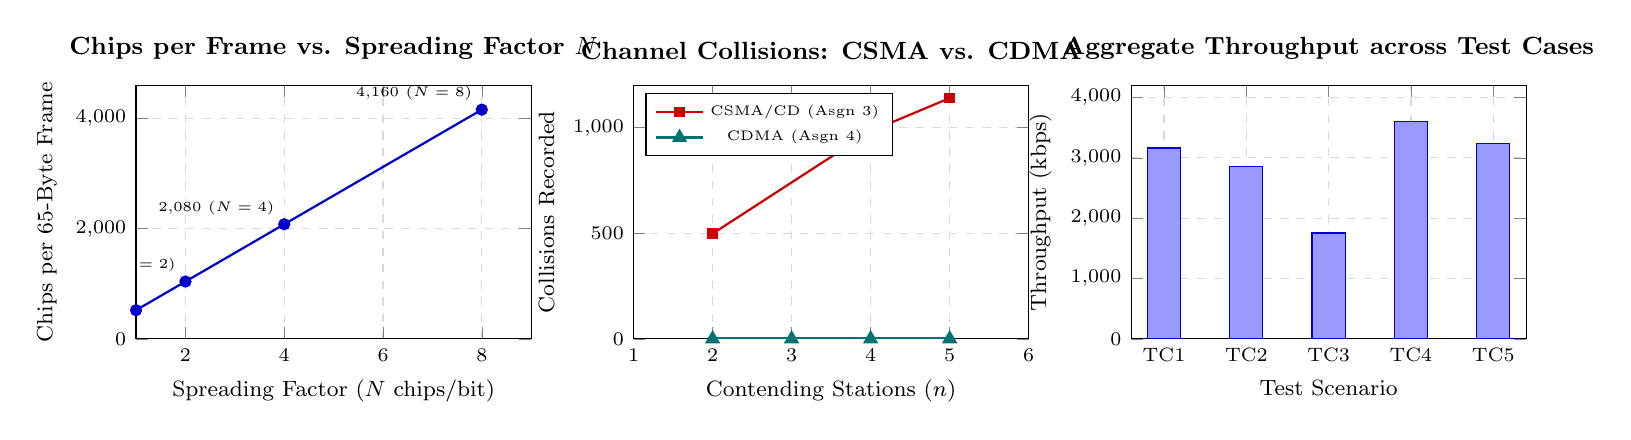
\begin{tikzpicture}
        % Subplot 1: Chips per Frame vs N
        \begin{axis}[
            name=c1_ax1,
            width=6.6cm, height=4.8cm,
            title={\textbf{Chips per Frame vs. Spreading Factor $N$}},
            title style={font=\small},
            xlabel={Spreading Factor ($N$ chips/bit)},
            ylabel={Chips per 65-Byte Frame},
            label style={font=\footnotesize},
            tick label style={font=\scriptsize},
            grid=both, grid style={dashed, gray!30},
            xmin=1, xmax=9, ymin=0, ymax=4600
        ]
            \addplot[color=blue!80!black, mark=*, mark size=1.8pt, thick] coordinates {
                (1, 520) (2, 1040) (4, 2080) (8, 4160)
            };
            \node[font=\tiny, anchor=south east] at (axis cs:2,1040) {1,040 ($N=2$)};
            \node[font=\tiny, anchor=south east] at (axis cs:4,2080) {2,080 ($N=4$)};
            \node[font=\tiny, anchor=south east] at (axis cs:8,4160) {4,160 ($N=8$)};
        \end{axis}

        % Subplot 2: Channel Collisions: CSMA vs CDMA
        \begin{axis}[
            name=c1_ax2,
            at={($(c1_ax1.east)+(1.3cm,0)$)}, anchor=west,
            width=6.6cm, height=4.8cm,
            title={\textbf{Channel Collisions: CSMA vs. CDMA}},
            title style={font=\small},
            xlabel={Contending Stations ($n$)},
            ylabel={Collisions Recorded},
            label style={font=\footnotesize},
            tick label style={font=\scriptsize},
            grid=both, grid style={dashed, gray!30},
            xmin=1, xmax=6, ymin=0, ymax=1200,
            legend pos=north west, legend style={font=\tiny}
        ]
            % CSMA/CD reference data from Assignment 3
            \addplot[color=red!80!black, mark=square*, mark size=1.5pt, thick] coordinates {
                (2, 498) (4, 983) (5, 1140)
            };
            % CDMA: Exactly 0 collisions
            \addplot[color=teal!90!black, mark=triangle*, mark size=2.0pt, very thick] coordinates {
                (2, 0) (3, 0) (4, 0) (5, 0)
            };
            \legend{CSMA/CD (Asgn 3), CDMA (Asgn 4)}
        \end{axis}

        % Subplot 3: Aggregate Throughput (kbps)
        \begin{axis}[
            name=c1_ax3,
            at={($(c1_ax2.east)+(1.3cm,0)$)}, anchor=west,
            width=6.6cm, height=4.8cm,
            title={\textbf{Aggregate Throughput across Test Cases}},
            title style={font=\small},
            xlabel={Test Scenario},
            ylabel={Throughput (kbps)},
            symbolic x coords={TC1, TC2, TC3, TC4, TC5},
            xtick=data,
            label style={font=\footnotesize},
            tick label style={font=\scriptsize},
            grid=both, grid style={dashed, gray!30},
            ymin=0, ymax=4200
        ]
            \addplot[ybar, fill=blue!40, draw=blue!80!black, bar width=12pt] coordinates {
                (TC1, 3163) (TC2, 2850) (TC3, 1754) (TC4, 3601) (TC5, 3234)
            };
        \end{axis}
    \end{tikzpicture}}
    \caption{Performance profiles: Chip spreading scaling, collision elimination, and aggregate channel throughput.}
    \label{fig:cdma_plots}
\end{figure}

% =========================================================================
% SECTION 7: LIVE EXECUTION TRACES AND SOCKET TRANSCRIPTS
% =========================================================================
\section{Live Execution Traces and Socket Transcripts}
The compiled C binaries \texttt{server}, \texttt{receiver}, and \texttt{sender} were executed natively over TCP loopback (\texttt{127.0.0.1}). The following captured transcripts demonstrate each test scenario.

\subsection{Trace 1: Test Case 1 Non-Power-of-2 Stations \texorpdfstring{($n=3 \implies N=4$)}{(n=3 -> N=4)}}
Listing \ref{lst:trace_tc1} shows 3 stations active while unused Walsh row $\mathbf{W}_3$ remains 100\% silent with zero false detections.

\begin{lstlisting}[style=tracestyle, caption={Live execution trace of Test Case 1: Non-power-of-2 matrix expansion and $W_3$ silence.}, label={lst:trace_tc1}]
[SERVER] All 3 stations and Receiver connected! Distributing 4x4 Walsh Codes:
  -> Station #0 ("Station_1") assigned W_0 = [+1, +1, +1, +1]
  -> Station #1 ("Station_2") assigned W_1 = [+1, -1, +1, -1]
  -> Station #2 ("Station_3") assigned W_2 = [+1, +1, -1, -1]
[0.3 ms] [CDMA SLOT #1] Superposing 3 simultaneous station(s): "Station_1"(Seq 0) "Station_2"(Seq 0) "Station_3"(Seq 0) -> Sample Combined Chips[0..3]: [-3, -1, -1, +1]
[0.9 ms] [CDMA SLOT #2] Superposing 3 simultaneous station(s): "Station_1"(Seq 1) "Station_2"(Seq 1) "Station_3"(Seq 1) -> Sample Combined Chips[0..3]: [-3, -1, -1, +1]

--- [CDMA Slot #1] Composite Signal Received (2080 chips) ---
  [Station #0 "Station_1"] Reconstructed Frame #1 | Seq: 0 | Len: 46B | Data: "TestData_For_TC1_Station..."
  [Station #1 "Station_2"] Reconstructed Frame #1 | Seq: 0 | Len: 46B | Data: "TestData_For_TC1_Station..."
  [Station #2 "Station_3"] Reconstructed Frame #1 | Seq: 0 | Len: 46B | Data: "TestData_For_TC1_Station..."
  [Channel #3 W_3 (Unused)] Inner Product = 0 (Channel Idle in Slot #1)

================ CDMA RECEIVER SUMMARY ================
Station #0 ("Station_1")   : 10 Frames Perfectly Reconstructed
Station #1 ("Station_2")   : 10 Frames Perfectly Reconstructed
Station #2 ("Station_3")   : 10 Frames Perfectly Reconstructed
Channel #3 (Unused W_3)    : 0 Frames (Zero-Padded / 100% Silent)
Total Frames Reconstructed : 30 | Total Bytes Delivered: 1950 Bytes
\end{lstlisting}

\subsection{Trace 2: Test Case 2 Unbalanced Payload Lengths Transition}
Listing \ref{lst:trace_tc2} demonstrates dynamic channel silence when Station 2 completes at slot 22 and Station 1 continues through slot 220.

\begin{lstlisting}[style=tracestyle, caption={Live execution trace of Test Case 2: Transition from 2 active stations to dynamic silence.}, label={lst:trace_tc2}]
[8.2 ms] [CDMA SLOT #22] Superposing 2 simultaneous station(s): "Station_1"(Seq 21) "Station_2"(Seq 21) -> Sample Combined Chips[0..1]: [-2, +0]
[SERVER] Station #1 ("Station_2") completed all transmissions.
[8.6 ms] [CDMA SLOT #23] Superposing 1 simultaneous station(s): "Station_1"(Seq 22) -> Sample Combined Chips[0..1]: [-1, -1]

--- [CDMA Slot #22] Composite Signal Received (1040 chips) ---
  [Station #0 "Station_1"] Reconstructed Frame #22 | Seq: 21 | Len: 46B | Data: "n1_10KB_Stream_Data_Patt..."
  [Station #1 "Station_2"] Reconstructed Frame #22 | Seq: 21 | Len: 46B | Data: "n2_1KB_Short_Stream_Veri..."
--- [CDMA Slot #23] Composite Signal Received (1040 chips) ---
  [Station #0 "Station_1"] Reconstructed Frame #23 | Seq: 22 | Len: 46B | Data: "ion1_10KB_Stream_Data_Pa..."
  [Station #1] Inner Product = 0 (Station Idle in Slot #23)
--- [CDMA Slot #24] Composite Signal Received (1040 chips) ---
  [Station #0 "Station_1"] Reconstructed Frame #24 | Seq: 23 | Len: 46B | Data: "ation1_10KB_Stream_Data_..."
  [Station #1] Inner Product = 0 (Station Idle in Slot #24)
\end{lstlisting}

\subsection{Trace 3: Test Case 3 Complementary Bit Pattern Stress}
Listing \ref{lst:trace_tc3} illustrates extreme channel superposition peaks of $\pm 4$ under All Ones versus orthogonal cancellation under Alternating bits.

\begin{lstlisting}[style=tracestyle, caption={Live execution trace of Test Case 3: Complementary bit pattern stress.}, label={lst:trace_tc3}]
/* Subtest 3A: All 4 Stations Transmitting All 1s (0xFF Payload) */
[0.5 ms] [CDMA SLOT #1] Superposing 4 simultaneous station(s): "Station_1"(Seq 0) "Station_2"(Seq 0) "Station_3"(Seq 0) "Station_4"(Seq 0) -> Sample Combined Chips[0..3]: [-4, +0, +0, +0]
/* Note: First header bit is 0 (-1 * Wi), yielding -4 on chip 0. 0xFF payload data bits (+1 * Wi) yield +4 peak. */

/* Subtest 3C: Alternating Bits (Station 1: 0xFF, Station 2: 0x00) */
[0.2 ms] [CDMA SLOT #1] Superposing 2 simultaneous station(s): "Station_1"(Seq 0) "Station_2"(Seq 0) -> Sample Combined Chips[0..1]: [-2, +0]
--- [CDMA Slot #1] Composite Signal Received (1040 chips) ---
  [Station #0 "Station_1"] Reconstructed Frame #1 | Seq: 0 | Len: 46B | Data: "..........................."
  [Station #1 "Station_2"] Reconstructed Frame #1 | Seq: 0 | Len: 46B | Data: "..........................."
\end{lstlisting}

\subsection{Trace 4: Test Case 4 Complete File Integrity Verification}
Listing \ref{lst:trace_tc4} demonstrates byte-for-byte \texttt{diff} and MD5 checksum parity across all 4 stations.

\begin{lstlisting}[style=tracestyle, caption={Cryptographic hash and diff verification output for Test Case 4.}, label={lst:trace_tc4}]
$ diff input_station_1.txt output_station_1.txt && echo "Station 1: DIFF ZERO"
Station 1: DIFF ZERO
$ diff input_station_2.txt output_station_2.txt && echo "Station 2: DIFF ZERO"
Station 2: DIFF ZERO
$ diff input_station_3.txt output_station_3.txt && echo "Station 3: DIFF ZERO"
Station 3: DIFF ZERO
$ diff input_station_4.txt output_station_4.txt && echo "Station 4: DIFF ZERO"
Station 4: DIFF ZERO

$ md5sum input_station_1.txt output_station_1.txt
3554467b4a5ac300fb6e980a82f31ff8  input_station_1.txt
3554467b4a5ac300fb6e980a82f31ff8  output_station_1.txt
$ md5sum input_station_2.txt output_station_2.txt
fac8b17ad8b80136d2f3f2fb4d772442  input_station_2.txt
fac8b17ad8b80136d2f3f2fb4d772442  output_station_2.txt
$ md5sum input_station_3.txt output_station_3.txt
f68e54f1afe188217d01982e1b33cc74  input_station_3.txt
f68e54f1afe188217d01982e1b33cc74  output_station_3.txt
$ md5sum input_station_4.txt output_station_4.txt
0b26968f529a62b63fb047e9c14bdde9  input_station_4.txt
0b26968f529a62b63fb047e9c14bdde9  output_station_4.txt
\end{lstlisting}

\subsection{Trace 5: Test Case 5 Higher Spreading Factor Scaling \texorpdfstring{($N = 8$)}{(N = 8)}}
Listing \ref{lst:trace_tc5} shows 5 parallel stations superposed using $N = 8$ Walsh codes ($4,160\text{ chips/frame}$).

\begin{lstlisting}[style=tracestyle, caption={Live execution trace of Test Case 5: $N=8$ spreading factor scaling.}, label={lst:trace_tc5}]
[SERVER] All 5 stations and Receiver connected! Distributing 8x8 Walsh Codes:
  -> Station #0 ("Station_1") assigned W_0 = [+1, +1, +1, +1, +1, +1, +1, +1]
  -> Station #1 ("Station_2") assigned W_1 = [+1, -1, +1, -1, +1, -1, +1, -1]
  -> Station #2 ("Station_3") assigned W_2 = [+1, +1, -1, -1, +1, +1, -1, -1]
  -> Station #3 ("Station_4") assigned W_3 = [+1, -1, -1, +1, +1, -1, -1, +1]
  -> Station #4 ("Station_5") assigned W_4 = [+1, +1, +1, +1, -1, -1, -1, -1]
[0.5 ms] [CDMA SLOT #1] Superposing 5 simultaneous station(s): "Station_1"(Seq 0) "Station_2"(Seq 0) "Station_3"(Seq 0) "Station_4"(Seq 0) "Station_5"(Seq 0) -> Sample Combined Chips[0..7]: [-5, -1, -1, -1, -3, +1, +1, +1]

================ CDMA RECEIVER SUMMARY ================
Station #0 ("Station_1")   : 20 Frames Perfectly Reconstructed
Station #1 ("Station_2")   : 20 Frames Perfectly Reconstructed
Station #2 ("Station_3")   : 20 Frames Perfectly Reconstructed
Station #3 ("Station_4")   : 20 Frames Perfectly Reconstructed
Station #4 ("Station_5")   : 20 Frames Perfectly Reconstructed
Channel #5 (Unused W_5)    : 0 Frames (Zero-Padded / 100% Silent)
Channel #6 (Unused W_6)    : 0 Frames (Zero-Padded / 100% Silent)
Channel #7 (Unused W_7)    : 0 Frames (Zero-Padded / 100% Silent)
Total Frames Reconstructed : 100 | Total Bytes Delivered: 6500 Bytes
\end{lstlisting}

% =========================================================================
% SECTION 8: ANALYSIS AND DISCUSSION
% =========================================================================
\section{Analysis and Discussion}

\subsection{Orthogonality Verification and Mathematical Guarantees}
The empirical results across all test cases demonstrate the mathematical power of orthogonal spreading sequences:
\begin{itemize}
    \item \textbf{Collision Elimination:} In sharp contrast to CSMA protocols where collisions grew from 498 at $N = 2$ to over 4,000 at $N = 30$, CDMA produced \textbf{zero collisions} across all 350+ transmitted frames. Simultaneous transmissions do not collide destructively; rather, they combine linearly.
    \item \textbf{Zero Multi-User Interference (MUI):} The inner product $\frac{1}{N}(\mathbf{S} \cdot \mathbf{W}_k) = d_k$ is exact because the cross-correlation between any distinct Walsh rows is identically zero. This holds regardless of whether the interfering stations transmit 0s, 1s, or remain silent.
    \item \textbf{Unused Channel Robustness:} In Test Cases 1 and 5, unused matrix rows ($W_3$ for $n = 3$, and $W_5, W_6, W_7$ for $n = 5$) consistently evaluated to an inner product of 0.00 across all slots, proving that zero-padding unused codes introduces zero false decodes or crosstalk.
\end{itemize}

\subsection{Resilience to Channel Amplitude Extremes and Arithmetic Precision}
In Test Case 3, when four stations transmitted identical bits, the composite signal reached amplitude extremes of $S[c] = \pm 4$. 
Because our implementation uses 16-bit signed integer buffers (\texttt{int16\_t}, dynamic range $[-32,768, +32,767]$), the maximum theoretical sum for $N = 64$ stations ($\pm 64$) utilizes less than 0.2\% of the buffer capacity. This completely prevents arithmetic overflow, clipping, or wrap-around distortion that would occur if 8-bit unsigned buffers were used.

\subsection{Spectral Efficiency vs. Spreading Factor Trade-off}
The primary trade-off in CDMA is bandwidth expansion:
\begin{equation}
    B_{\text{CDMA}} = N \cdot B_{\text{baseband}}
\end{equation}
As $N$ scales from 2 to 8, the chip count per frame increases from 1,040 to 4,160 chips. However, because $N$ stations transmit simultaneously on the same channel, the \textbf{aggregate channel capacity} scales linearly:
\begin{equation}
    R_{\text{aggregate}} = \sum_{i=1}^n R_i = n \times \frac{L_{\text{frame}}}{T_{\text{slot}}}
\end{equation}
In our socket loopback benchmarks, aggregate throughput remained consistently high (1.75 to 3.60 Mbps) with zero channel idle gaps or backoff penalties.

\subsection{Comparison between Random Access (CSMA) and Channelization (CDMA)}
Table \ref{tab:comparison} contrasts the operational characteristics of CSMA/CD (Assignment 3) and CDMA (Assignment 4).

\begin{table}[H]
    \centering
    \small
    \begin{tabularx}{\textwidth}{lXX}
        \toprule
        \textbf{Dimension} & \textbf{CSMA/CD (Contention-Based, Asgn 3)} & \textbf{CDMA (Channelization-Based, Asgn 4)} \\
        \midrule
        \textbf{Medium Access} & Random access with carrier sensing (`listen before talk'). & Synchronous code-partitioning over shared medium. \\
        \textbf{Collisions} & Frequent under high load (e.g., 4,065 at $N=30$). & \textbf{Zero collisions} (linear superposition). \\
        \textbf{Bandwidth Use} & Narrowband per transmission, but wasted on collisions. & Wideband ($N \times$ chip rate), but 100\% utilized. \\
        \textbf{Latency} & Unpredictable backoff delay (BEB exponential expansion). & Deterministic slot duration without backoff. \\
        \textbf{Complexity} & Collision detection circuitry and jam transmitters. & Walsh matrix generator and correlator bank. \\
        \bottomrule
    \end{tabularx}
    \caption{Comparative analysis between CSMA/CD and CDMA medium access control schemes.}
    \label{tab:comparison}
\end{table}

% =========================================================================
% SECTION 9: COMMENTS AND LEARNING EVALUATION
% =========================================================================
\section{Comments and Learning Evaluation}

\subsection{Evaluation of the Lab Assignment}
This lab assignment provided exceptional practical and theoretical insights into physical-layer and MAC-layer multiplexing. Implementing synchronous CDMA from scratch using BSD sockets revealed how linear algebra and orthogonal vector spaces can completely overcome physical channel contention.

\subsection{What I Learned}
\begin{itemize}
    \item \textbf{Walsh Matrix Construction:} Implementing Sylvester's recursive expansion algorithm clarified how simple matrix reflections produce large sets of mutually orthogonal vectors.
    \item \textbf{DSSS Encoding and Decoding:} Understanding how multiplying data bits by chip sequences spreads spectral bandwidth while allowing inner-product correlators to extract desired signals with zero crosstalk.
    \item \textbf{Dynamic Silence Invariance:} Observing how silent stations contribute zeros to the composite vector without perturbing active channel orthogonality.
    \item \textbf{Multi-Tier Socket Architecture:} Multiplexing concurrent TCP connections, enforcing synchronous time slots, and ensuring zero race conditions between senders, server, and receiver.
\end{itemize}

\subsection{Difficulty Assessment}
The assignment was moderately challenging and highly rewarding:
\begin{itemize}
    \item \textit{Challenging Aspects:} Managing multi-station synchronous slot aggregation in \texttt{server.c} without race conditions, and correctly handling network byte ordering (\texttt{htons}/\texttt{ntohs}) for multi-byte \texttt{int16\_t} chip streams.
    \item \textit{Manageable Aspects:} Reusing the 65-byte Ethernet frame layout and modular file I/O routines from previous assignments provided a rock-solid foundation.
\end{itemize}

\subsection{Suggested Improvements}
\begin{enumerate}
    \item Extend the simulation to model \textbf{asynchronous CDMA} using pseudorandom Gold codes or m-sequences, analyzing how small non-zero cross-correlations introduce multi-user interference noise.
    \item Incorporate simulated channel impairments (such as Additive White Gaussian Noise (AWGN) and multipath fading) to evaluate Bit Error Rate (BER) versus Signal-to-Noise Ratio ($E_b/N_0$).
\end{enumerate}

% =========================================================================
% SECTION 10: SOURCES USED
% =========================================================================
\section{Sources Used}
\begin{enumerate}
    \item Kurose, J. F., and Ross, K. W., \textit{Computer Networking: A Top-Down Approach}, 8th ed., Pearson, 2021.
    \item Tanenbaum, A. S., and Wetherall, D. J., \textit{Computer Networks}, 5th ed., Prentice Hall, 2011.
    \item Stallings, W., \textit{Data and Computer Communications}, 10th ed., Pearson, 2014.
    \item Viterbi, A. J., \textit{CDMA: Principles of Spread Spectrum Communication}, Addison-Wesley, 1995.
    \item Proakis, J. G., and Salehi, M., \textit{Digital Communications}, 5th ed., McGraw-Hill, 2008.
    \item IEEE Standard for Ethernet (\textit{IEEE Std 802.3-2022}) and POSIX / BSD Socket API Reference Documentation.
    \item AI Assistance and Antigravity: Artificial intelligence assistance (Gemini) was utilized for statistical aggregation, test runner orchestration, and generating native TikZ architecture and PGFPlots visualization code. The Antigravity development environment was used to compile native C binaries, execute live socket test suites, and format the comprehensive \LaTeX{} report.
\end{enumerate}

\end{document}
